\section{整型数据}

\begin{frame}\ft{整数的存储方式}
  \begin{itemize}
  \item 数据都是以二进制的形式存储。\vspace{0.1in}
  \item 整数以\red{补码}的方式存储。\vspace{0.1in}

    \begin{enumerate}
    \item
      正数的补码是其本身\\[0.1in]
    \item 
      负数的补码:将其绝对值的二进制形式按位取反再加1。
    \end{enumerate}

  \end{itemize}
\end{frame}
%
\begin{frame}\ft{整数的存储方式}

  \begin{figure}
    \centering
    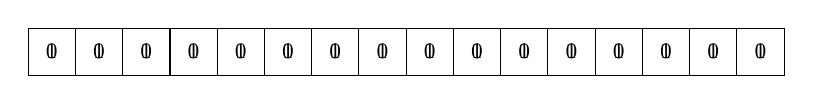
\begin{tikzpicture}
      \def\x{0.6}
      \foreach \i in {0,1,...,15}{
        \draw (-\i*\x,0)rectangle(-\i*\x-\x,\x);
        \ifthenelse{\i=1 \OR \i=3}
        {
          \node at (-\i*\x-0.5*\x,0.5*\x)[]{\footnotesize{1}};
        }
        {
          \node at (-\i*\x-0.5*\x,0.5*\x)[]{\footnotesize{0}};

        }
      }
    \end{tikzpicture}
    \caption{正数10的存储方式}
  \end{figure}
  % 
  \begin{figure}
    \centering
    \begin{tikzpicture}
      \def\x{0.6}
      \foreach \i in {0,1,...,15}{
        \draw (-\i*\x,0)rectangle(-\i*\x-\x,\x);
        \ifthenelse{\i=1 \OR \i=3}
        {
          \node at (-\i*\x-0.5*\x,0.5*\x)[]{\footnotesize{1}};
        }
        {
          \node at (-\i*\x-0.5*\x,0.5*\x)[]{\footnotesize{0}};
        }
      }
      \node at (-16*\x,1.3*\x) [right]{\footnotesize{10的原码}};
      %%%% 
      \foreach \i in {0,1,...,15}{
        \draw (-\i*\x,-2*\x)rectangle(-\i*\x-\x,-\x);
        \ifthenelse{\i=1 \OR \i=3}
        {
          \node at (-\i*\x-0.5*\x,-1.5*\x)[]{\footnotesize{0}};
        }
        {
          \node at (-\i*\x-0.5*\x,-1.5*\x)[]{\footnotesize{1}};
        }
      }
      \node at (-16*\x,-0.7*\x) [right]{\footnotesize{取反}};
      %%%% 
      \foreach \i in {0,1,...,15}{
        \draw (-\i*\x,-4*\x)rectangle(-\i*\x-\x,-3*\x);
        \ifthenelse{\i=0 \OR \i=3}
        {
          \node at (-\i*\x-0.5*\x,-3.5*\x)[]{\footnotesize{0}};
        }
        {
          \node at (-\i*\x-0.5*\x,-3.5*\x)[]{\footnotesize{1}};
        }
      }
      \node at (-16*\x,-2.7*\x) [right]{\footnotesize{加1,得-10的补码}};

    \end{tikzpicture}
    \caption{负数-10的存储方式}
  \end{figure}
\end{frame}

\begin{frame}[fragile]\ft{ \lst|int| 型}
  \lst|int| 型表示有符号整数,其取值范围依赖于系统。
  \begin{itemize}
  \item C:使用头文件 \lst|limits.h|
    \begin{itemize}
    \item 它专用于检测\red{整型数据类型}的取值范围。
    \end{itemize}
  \item C++:使用头文件 \lst|limits|
    \begin{itemize}
    \item 它提供了 \lst|std::numeric_limits| 模板类,用于替代C语言,检测\red{各种基本数据类型}的取值范围及其他信息。
    \end{itemize}
  \end{itemize}
\end{frame}
%
\begin{frame}[fragile]\ft{ \lst|int| 型}
  \lstinputlisting[basicstyle=\ttfamily\small]
  {slide03/code/int_info.c}
\pause 
\begin{lstlisting}[backgroundcolor=\color{red!10}]
$ gcc  int_info.c
$ ./a.out
range of int is -2147483648 ~ 2147483647
sizeof int = 4 bytes
\end{lstlisting}
\end{frame}

\begin{frame}[fragile]\ft{ \lst|int| 型}
  \lstinputlisting[basicstyle=\ttfamily\small]
  {slide03/code/int_info.cpp}
\pause 
\begin{lstlisting}[backgroundcolor=\color{red!10}]
$ g++  int_info.cpp
$ ./a.out
range of int is -2147483648 ~ 2147483647
sizeof int = 4 bytes
\end{lstlisting}
\end{frame}


\begin{frame}[fragile]\ft{ \lst|int| 变量的声明}
关键字 \lst|int| 用于声明基本的整型变量,书写格式为
\begin{lstlisting}[language=c,backgroundcolor=\color{red!10}]
int var;
int var1, var2;
\end{lstlisting}  \vspace{0.05in}

要声明多个变量,\vspace{0.05in}
\begin{itemize}
\item 可以逐个声明每个变量;\\[0.1in]
\item 也可在 \lst|int| 后跟一个变量名列表,各个变量之间用逗号隔开。
\end{itemize}

\end{frame}
% %
\begin{frame}[fragile]\ft{ \lst|int| 变量的赋值}
 \lst|int| 变量的赋值有如下三种方式:\vspace{0.05in}
\begin{enumerate}
\item 先声明,后赋值
\begin{lstlisting}
int n;
n = 1;
\end{lstlisting}
\item 先声明,后通过scanf函数赋值
\begin{lstlisting}
int n;
scanf("%d", &n);
\end{lstlisting} 
\item 初始化变量
\begin{lstlisting}
int n = 1;
\end{lstlisting} 
\end{enumerate}
\end{frame}
%
%
\begin{frame}[fragile]\ft{ \lst|int| 变量的初始化}
初始化变量就是为变量赋一个初始值。
\begin{lstlisting}[language=c,backgroundcolor=\color{red!10}]
int a = 1;
int b = 2, c = 3;
int d, e = 4;  // valid, but not good
\end{lstlisting}
请避免在一个声明语句中同时出现初始化和未初始化的变量。
\end{frame}
%
\begin{frame}[fragile]\ft{ \lst|int| 变量的初始化}
声明语句为变量创建、标定存储空间并为其指定初始值。 \pause 

\begin{figure}
\centering
\begin{tikzpicture}
\def\x{1}
\def\d{0}
\draw[thick,fill=gray!20] (0,\d)rectangle(5*\x,\d+0.5*\x);
\draw(2*\x,\d+0)--(2*\x,\d+0.5*\x);
\draw(3*\x,\d+0)--(3*\x,\d+0.5*\x);
\node at (2.5*\x,\d) [below] {b}; 
\node at (2.5*\x,\d+0.25*\x) [] {2}; 
\coordinate (b) at (-4*\x,\d);
\node at (b)  [above]{ \lst|int|  b=2;};
\draw[thick,->,>=stealth] (b) -- ++(0,-\x) -- 
node[above]{\footnotesize{分配存储空间并赋值}}
++(6.5*\x,0) -- ++(0,0.5*\x);

\def\d{2*\x}
\draw[thick,fill=gray!20] (0,\d)rectangle(5*\x,\d+0.5*\x);
\draw(2*\x,\d+0)--(2*\x,\d+0.5*\x);
\draw(3*\x,\d+0)--(3*\x,\d+0.5*\x);
\node at (2.5*\x,\d) [below] {a}; 
\coordinate (a) at (-4*\x,\d);
\node at (a)  [above]{ \lst|int|  a;};
\draw[thick,->,>=stealth] (a) -- ++(0,-\x) -- 
node[above]{\footnotesize{分配存储空间}}
++(6.5*\x,0) -- ++(0,0.5*\x);
\end{tikzpicture}
\caption{定义和初始化变量}
\end{figure}


\end{frame}
%
%
\begin{frame}[fragile]\ft{ \lst|int| 值的打印}
  \lstinputlisting[basicstyle=\ttfamily\small]
  {slide03/code/print1.c} 
\pause 

\begin{lstlisting}[backgroundcolor=\color{red!10}]
$ gcc print1.c
$ ./a.out
Doing it right: 10 - 2 = 8
Doing it wrong: 10 - 73832 = 771
\end{lstlisting}
\end{frame}
%
%
\begin{frame}[fragile]\ft{ \lst|int| 值的打印}

 第二次调用 \lst|print()| 时,程序使用 \lst|a| 为第一个 \lst|%d| 提供打印值,然后用内存中的任意值为其余两个 \lst|%d| 提供打印值。\vspace{0.1in}

 \begin{free}[注意]{}
   使用 \lst|printf()| 时,格式说明符的个数与要显示值的数目必须相同。
 \end{free}

 
\end{frame}
% %
% %
\begin{frame}[fragile]\ft{八进制数和十六进制数的打印}
在C中,有专门的前缀指明进制。

\begin{itemize}
\item 前缀 \lst|0x| 或 \lst|0X| 表示十六进制数\\[0.1in]
  \begin{itemize}
  \item \lst|16| 的十六进制表示为 \lst|0x10| 或 \lst|0X10|。\\[0.2in]
  \end{itemize}
\item 前缀 \lst|0| 表示八进制数\\[0.1in]
  \begin{itemize}
  \item \lst|16| 的八进制表示为 \lst|020|。
  \end{itemize}
\end{itemize}
\end{frame}

\begin{frame}[fragile]\ft{打印八进制数和十六进制数}
\lstinputlisting[language=c,frame=single,numbers=left]{
slide03/code/bases.c
}
% \end{frame}
% %
% %
% \begin{frame}[fragile]\ft{八进制数和十六进制数的打印}
\pause 
\begin{lstlisting}[language=c,backgroundcolor=\color{red!10}]
$ gcc bases.c
$ ./a.out
dec = 100; oct = 144; hex = 64
dec = 100; oct = 0144; hex = 0x64
\end{lstlisting}
\end{frame}
%
\begin{frame}[fragile]\ft{八进制数和十六进制数的打印}
\begin{table}
\centering
\begin{tabular}{p{2cm}|p{2cm}|p{4cm}} \hline
进制&格式说明符&格式说明符(显示前缀)\\\hline
十进制& \lst|%d| & \\
八进制& \lst|%o| & \lst|%#o|\\
十六进制& \lst|%x| 或 \lst|%X|  & \lst|%#x| 或 \lst|%#X|\\\hline
\end{tabular}
\end{table}
\end{frame}
% %
\begin{frame}[fragile]\ft{其他整数类型}
C/C++提供4个附属关键字修饰 \lst|int| :\lst|short|、\lst|long|、\lst|unsigned| 和 \lst|signed|。

\begin{table}
\centering
\begin{tabular}{p{4.5cm}|p{3cm}|p{2.8cm}} \hline
类型&含义&占位符\\\hline
\lst|short (int)|&   适用于小数值 &  \lst|%hd, %ho, %hx|\\[0.1in]\hline
\lst|long (int)| &   适用于大数值 &  \lst|%ld, %lo, %lx|\\[0.1in]\hline
\lst|long long (int)|& 适用于更大数值&  \lst|%lld, %llo, %llx|  \\
\hline
\lst|unsigned (int)|&    & \lst|%u|\\[0.1in]\hline
\lst|unsigned long (int)| &   & \lst|%lu| \\[0.1in]\hline
\lst|unsigned long long (int)|   &  &\lst|%llu|\\
\hline
\end{tabular}
\end{table}
\pause

关键字signed可以和任何有符号类型一起使用,使数据类型更加明确。
如short、short int、signed short和signed short int表示同一种类型。
\end{frame}
% %
\begin{frame}[fragile]\ft{其他数据类型}
  \begin{question}[]{}
    为什么会出现多种整数类型?
  \end{question}
  \pause 
  %C仅保证short类型不会比 \lst|int| 类型长,long类型不会比 \lst|int| 类型短,其目的是为了适应不同的机器。\vspace{0.05in}

  \begin{itemize}
  \item 有些CPU的自然字大小,若认为没有表示更大数的需要,会将long类型和 \lst|int| 类型定义相同的长度。\\[0.1in]
  \item 很多场合不要用到太大的整数,于是创建了更节省空间的short类型。
  \end{itemize}
\end{frame}

\begin{frame}[fragile]\ft{整数的上溢}
\begin{question}[]{}
若整数太大,超出整数类型的范围会发生什么?
\end{question}
\end{frame}

\begin{frame}[fragile]\ft{整数的上溢}
\lstinputlisting[language=c,frame=single,numbers=left]{
slide03/code/intOverflow.c
}
\end{frame}
%
\begin{frame}[fragile]\ft{整数的上溢}

\begin{lstlisting}[language=c,backgroundcolor=\color{red!10}]
$ gcc intOverflow.c
$ ./a.out
i = 2147483647, i+1 = -2147483648, i+2 = -2147483647
j = 4294967295, j+1 = 0, j+2 = 1
\end{lstlisting}
\end{frame}
%
\begin{frame}[fragile]\ft{整数的上溢}

当达到最大值时,将溢出到起始点。\vspace{0.05in}
\begin{itemize}
\item 对于unsigned int类型,起始点是0;\\[0.1in]
\item 对于int类型,起始点为-2147483648。
\end{itemize}

\vspace{0.1in}
 注意: 当整数溢出时,编译器不会给出任何提示,故编程时必须谨慎对待此类问题。 

\end{frame}
